


Although I was born in Madrid, Galicia (north of Spain) is a very
special region for me. More precisely, Cedeira and Valdoviño offer
a wonderful combination of wild sea, secluded beaches and
forests. I will show you a map of this marvelous places. 

The first step is to acquire information from the OpenStreetMap
project. There are several packages to extract data from this
service but, while most of them only provide already rendered
raster images, the \texttt{osmar} package enables the use of the raw data
with classes from the packages \texttt{sp} and \texttt{igraph}.

The \texttt{get\_osm} function retrieves a region defined by \texttt{corner\_bbox}
using the OSM API.


\lstset{language=R}
\begin{lstlisting}
library('osmar')

api <- osmsource_api()
ymax <- 43.7031
ymin <- 43.6181
xmax <- -8.0224
xmin <- -8.0808
box <- corner_bbox(xmin, ymin, xmax, ymax)
cedeira <- get_osm(box, source=api, full=TRUE)
\end{lstlisting}


The \texttt{cedeira} object includes three main components: nodes, ways
and relations. 
  

\lstset{language=R}
\begin{lstlisting}
summary(cedeira)
summary(cedeira$nodes)
\end{lstlisting}

These components can be accessed with the functions \texttt{find}, \texttt{subset}, \texttt{way},
\texttt{node}, \texttt{relation} and \texttt{tags}. Thus, the different kinds of roads
can be obtained using \texttt{way} and \texttt{tags} with the appropiate
tag. 


\lstset{language=R}
\begin{lstlisting}
idxHighways <- find(cedeira, way(tags(k=='highway')))
highways <- subset(cedeira, way_ids=idxHighways)
idxStreets <- find(highways, way(tags(v=='residential')))
idxPrimary <- find(highways, way(tags(v=='primary')))
idxSecondary <- find(highways, way(tags(v=='secondary')))
idxTertiary <- find(highways, way(tags(v=='tertiary')))
idxOther <- find(highways,
                 way(tags(v=='unclassified' |
                          v=='footway' |
                          v=='steps')))
\end{lstlisting}

The result of \texttt{find} is the index of each element. The
correspondent spatial object is extracted with \texttt{find\_down} and
\texttt{subset}, and can be converted to a class defined by the \texttt{sp}
package with \texttt{as\_sp}. The next \texttt{spFromOSM} function encodes the
procedure, and extracts the \texttt{SpatialLines} which represent each
type of road.


\lstset{language=R}
\begin{lstlisting}
spFromOSM <- function(source, index, type='lines'){
  idx <- find_down(source, index)
  obj <- subset(source, ids=idx)
  objSP <- as_sp(obj, type)
  }

streets <- spFromOSM(cedeira, way(idxStreets))
primary <- spFromOSM(cedeira, way(idxPrimary))
secondary <- spFromOSM(cedeira, way(idxSecondary))
tertiary <- spFromOSM(cedeira, way(idxTertiary))
other <- spFromOSM(cedeira, way(idxOther))
\end{lstlisting}
  
A similar procedure can be applied to construct a \texttt{SpatialPoints}
object with the collection of places with name:

\lstset{language=R}
\begin{lstlisting}
idxPlaces <- find(cedeira, node(tags(k=='name')))
places <- spFromOSM(cedeira, node(idxPlaces), 'points')

nms <- subset(cedeira$nodes$tags, subset=(k=='name'), select=c('id', 'v'))
ord <- match(idxPlaces, nms$id)
nms <- nms[ord,]
places$name <- nms$v[ord]
\end{lstlisting}

The second step is to produce a hill shade layer. This layer can
be computed from the slope and aspect layers derived from a
Digital Elevation Model. The DEM for this region is available at
the Geonetwork-SECAD service from the Universidad de Extremadura
and can be read with \texttt{raster}:

\lstset{language=R}
\begin{lstlisting}
## Galicia DEM
## http://ide.unex.es/geonetwork/srv/es/main.search?any=MDE_Galicia
## http://ide.unex.es:8180/geonetwork/srv/es/resources.get?id=21&fname=dem_gal.7z&access=private

old <- tempdir()
download.file('http://ide.unex.es:8180/geonetwork/srv/es/resources.get?id=21&fname=dem_gal.7z&access=private', 'dem_gal.7z')
unzip('dem_gal.7z')
demGalicia <- raster('dem_gal.asc')
setwd(old)
\end{lstlisting}



The \texttt{slope} and \texttt{aspect} layers are computed with the \texttt{terrain}
function, and the hill shade layer is derived with these layers
for a fixed sun position. Previously, the useful region of the DEM
raster is extracted with the \texttt{crop}:


\lstset{language=R}
\begin{lstlisting}
cedeiraSP <- as_sp(cedeira, 'points')
projCedeira <- projection(cedeiraSP)
##extCedeira <- bbox(cedeiraSP) 
## or summary(cedeira$nodes)$bbox
extCedeira <- extent(-8.15, -7.95, 43.6, 43.75)
demCedeira <- crop(demGalicia, extCedeira)
projection(demCedeira) <- projCedeira
demCedeira[demCedeira <= 0] <- NA

slope <- terrain(demCedeira, 'slope')
aspect <- terrain(demCedeira, 'aspect')
hsCedeira <- hillShade(slope=slope, aspect=aspect,
                       angle=20, direction=30)
\end{lstlisting}

And finally, the third step is to display the different layers of
information in correct order: the hill shade layer, the roads, and
the places (points and labels).
  

\lstset{language=R}
\begin{lstlisting}
##Auxiliary function to display the roads. A thicker black line in
##the background and a thinner one with an appropiate color.
sp.road <- function(line, lwd=5, blwd=7,
                    col='indianred1', bcol='black'){
  sp.lines(line, lwd=blwd, col=bcol)
  sp.lines(line, lwd=lwd, col=col)
}

## The background color of the panel is set to blue to represent the sea
myTheme <- GrTheme()
myTheme$panel.background$col = 'skyblue3'



levelplot(hsCedeira, par.settings=myTheme, margin=FALSE, colorkey=FALSE)+
  layer(sp.road(streets, lwd=1, blwd=2, col='white')) +
  layer(sp.road(other, lwd=2, blwd=3, col='white')) +
  layer(sp.road(tertiary, lwd=3, blwd=4, col='palegreen')) +
  layer(sp.road(secondary, lwd=4, blwd=6, col='midnightblue')) +
  layer(sp.road(primary, col='indianred1')) +
  layer(sp.points(places, pch=19, col='black', cex=0.6, alpha=0.5)) +
  layer(sp.pointLabel(places, labels=places$name,
                      fontfamily = 'Palatino', 
                      cex=0.6, col='black'))
\end{lstlisting}

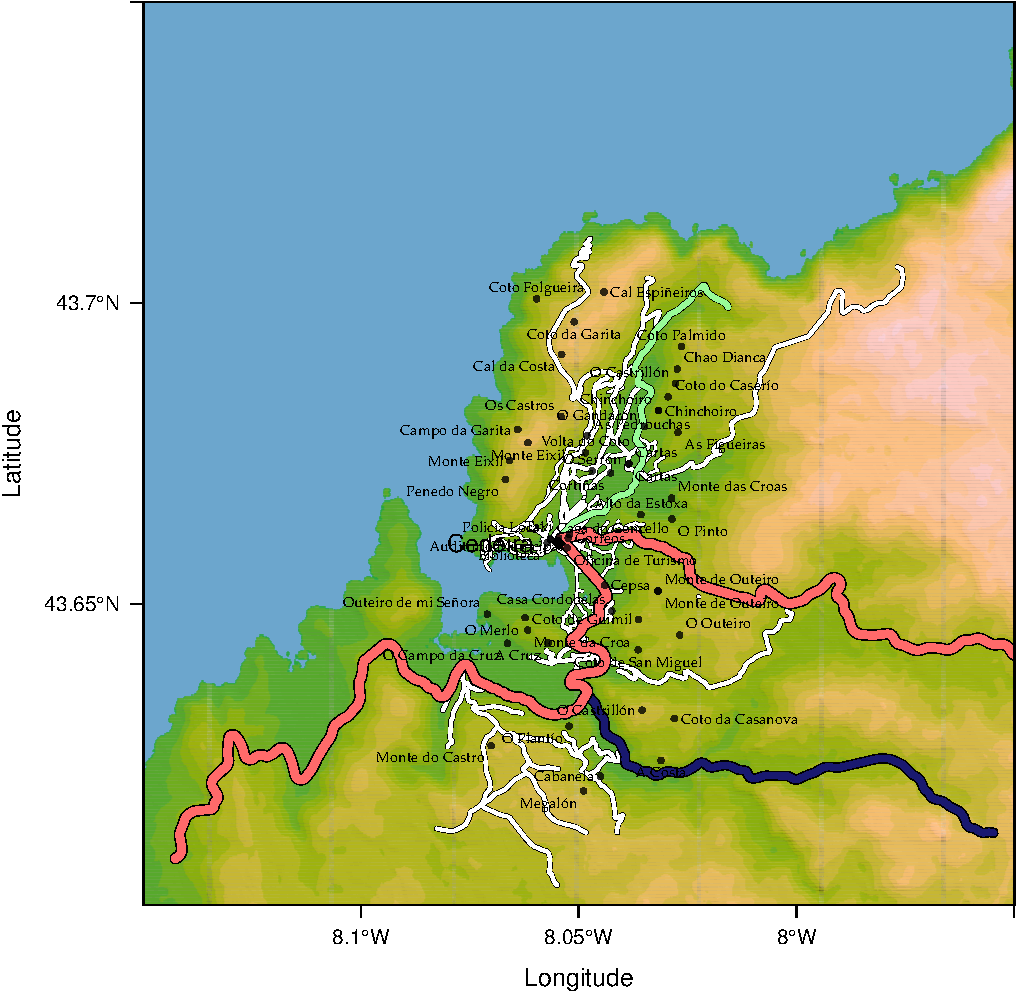
\includegraphics[width=.9\linewidth]{figs/cedeiraOsmar.pdf}




